\documentclass[10pt]{article}
\usepackage[margin=17mm]{geometry}
\usepackage{graphicx,booktabs,hyperref}
\usepackage[strings]{underscore}
\setlength{\parindent}{0pt}\setlength{\parskip}{4pt}
\begin{document}
\section*{Original fixtures: finite curve-membership audit}
Diagnostic date 2026-10-25. Source frozen at c470f5d51 before output.
The byte-identical original seven Boolean fixtures use GF($2^{22}$),
modulus $X^{22}+X+1$, and $E_0:y^2+xy=x^3+1$.
Exact input SHA-256 (two joined lines):\\
\texttt{95ee147e1221ce4ef6c98bdd0b808398}\\
\texttt{a01362343ffaa66debc217d6eeff5a9b}.

\begin{center}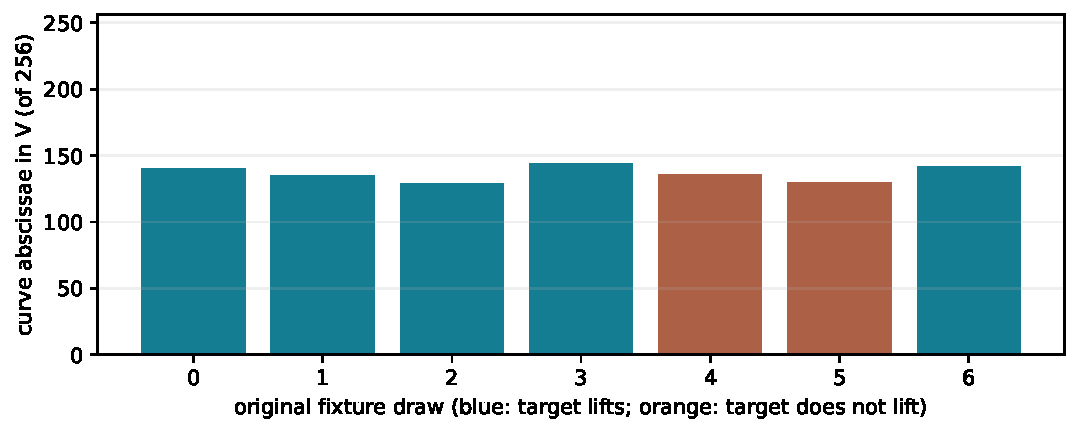
\includegraphics[width=.98\linewidth]{curve-lifts.pdf}\end{center}
\begin{center}\begin{tabular}{rrrrr}\toprule
Draw & Boolean solutions & target on curve & curve x in V & curve points in V\\\midrule
0 & 0 & yes & 140 & 279 \\
1 & 6 & yes & 135 & 269 \\
2 & 6 & yes & 129 & 257 \\
3 & 0 & yes & 144 & 287 \\
4 & 18 & no & 136 & 271 \\
5 & 0 & no & 130 & 259 \\
6 & 0 & yes & 142 & 283 \\
\bottomrule\end{tabular}\end{center}

The native audit finds 3/4
UNSAT targets and 2/3 SAT targets
liftable. Draws 4 and 5 are not ordinary curve-query abscissae for this model.
Draw 0, used by the all-eight balanced k=3 replay, is liftable.
This qualifies the application of these fixtures; it does not invalidate their
finite Boolean-system solution counts or refutation observations.

Every returned y root is checked by direct curve-equation substitution.
An independently evaluated Artin--Schreier trace criterion agrees for every
target and every element of each complete 256-element V. Counts include
x=0 and its two-torsion point. Neither target nor factor-base subgroup
membership is established. Curve membership alone does not prove a signed
point decomposition, a degree law, a complete DLP solve or a speed result.

Execution: native Rust, local shared x86-64 host; 12 GiB address-space cap,
900-second limit, exit 0, no timing comparison. A separate exhaustive
small-field test compares every y value at n=5,6,7; all three example tests pass.
Protocol: \path{../../FIXTURE_GROUP_PROTOCOL.md}.
Source: \path{examples/ic_fixture_group_audit.rs}.
Raw receipt and provenance: \path{../../pipeline-receipts/fixture-group-audit-20261025/}.
The old branch reports and source-pinned inputs are preserved unchanged.

\end{document}
